\documentclass[aspectratio=1610]{beamer}
\hypersetup{
        unicode=true,
        linkcolor=blue,
        anchorcolor=blue,
        citecolor=green,
        filecolor=black,
        urlcolor=blue
    }

%%%%% PACKAGES HERE
%% \usepackage{}
\usepackage{amsmath}
\usepackage{amssymb}
\usepackage{listings}
\usepackage[cache=false]{minted}
\usepackage{textcomp}
\usepackage[UTF8]{ctex} 

\usepackage[style=authortitle,backend=biber]{biblatex}
\addbibresource{references.bib}

\input{smile_styles}

%% Start from here.
\title{three paper: Antras}
\date\today

\begin{document}

\begin{frame}[plain]
  \titlepage
\end{frame}



\section{three paper: antras}

\begin{frame}
\centering
 \huge Introduction
\end{frame}

\begin{frame}{three paper}
\begin{enumerate}

    \item "Measuring the Average Period of Production" (joint with Vitalii Tubdenov), American Economic Association Papers and Proceedings, Vol. 115, May 2025, pp. 624–30).\vspace{1cm}
    \item "Interest Rates and World Trade: An ‘Austrian’ Perspective" American Economic Association Papers and Proceedings, Vol. 113, May 2023, pp. 65-69.\vspace{1cm}
    \item "An ʻAustrian’ Model of Global Value Chains" January 2023, reject and resubmit at the American Economic Review.
\end{enumerate}
    
\end{frame}


\begin{frame}{Austrian}
Austrian!


\end{frame}


\begin{frame}{Austrian}
Austrian!

\vspace{1cm}

Janek Wasserman’s “The Marginal Revolutionaries: How Austrian Economists Fought the War of Ideas” which inspired Antras to write this paper.

\end{frame}


\begin{frame}{Austrian}
Austrian!

\vspace{1cm}

Janek Wasserman’s “The Marginal Revolutionaries: How Austrian Economists Fought the War of Ideas” which inspired Antras to write this paper.

\vspace{1cm}

Production takes time.
\end{frame}


\begin{frame}{then, what research}
\begin{columns}[T]  % [T] 表示顶部对齐，默认居中 [c]
    \begin{column}{0.5\textwidth}  % 左栏占50%宽度
       \begin{figure}
           \centering
           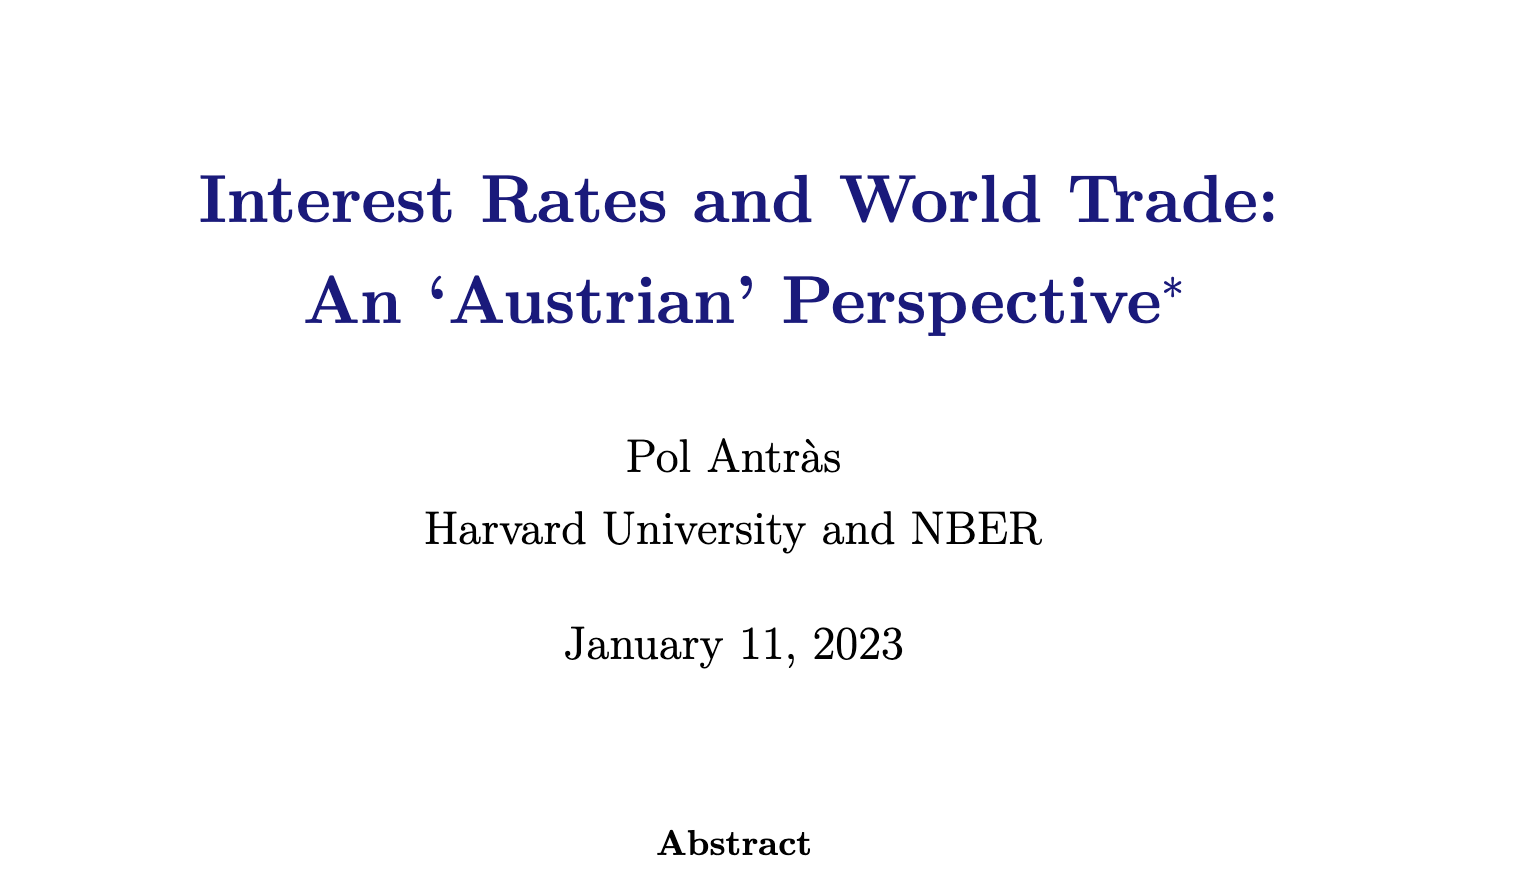
\includegraphics[width=\linewidth]{Figure3.png}
       \end{figure}
    \end{column}
    
    \begin{column}{0.5\textwidth}  % 右栏占50%宽度
    \begin{figure}
        \centering
        
\includegraphics[width=1\linewidth]{Figure5.png}
      
    \end{figure}
       \begin{figure}
           \centering
           
\includegraphics[width=1.5\linewidth]{Figure4.png}
         
       \end{figure}
       
    \end{column}
\end{columns}
    
\end{frame}


\begin{frame}{another one}
    \begin{figure}
        \centering
        
\includegraphics[width=1\linewidth]{Figure6.png}
    \end{figure}
\end{frame}

\begin{frame}
\centering
\huge Measuring the Average Period of Production
    
\end{frame}

\begin{frame}{Prodcution process}
a production take place in time interval[0,T]

\vspace{1cm}

$T$ :length of the prodcution process

\vspace{1cm}

the mapping between inputs and outputs, production function:
$$Y(\boldsymbol{L}) = Z(\boldsymbol{L}) F(\boldsymbol{L})$$

\vspace{1cm}

where, $$\boldsymbol{L} = \{\ell(t)\}_{t\in[0,T]}$$
$F(\boldsymbol{L})$: producution technology, homogeneous of degree one in $\boldsymbol{L} $

$Z(\boldsymbol{L})$: productivity, homogeneous of degree 0 in $\boldsymbol{L}$

\end{frame}

\begin{frame}{Production process}
define $\boldsymbol{\lambda} = \{\ell(t)/L\}_{t\in[0,T]}$, 

\vspace{1cm}

where $L = \int_{0}^{T} \ell(t) \, dt$, total labor use along the whole production process.

\vspace{1cm}
Thus, $\boldsymbol{\lambda}(t)$captures the distribution of labor expenditures along the production process.

\end{frame}

\begin{frame}{the measure!}
$$\mathcal{APP}(\boldsymbol{\lambda}) = \int_{0}^{T} (T-t)\lambda(t) \, dt.$$
    represents a weighted average temporal distance
\end{frame}

\begin{frame}{Relationship between APP and interest rates}
in the paper, long process
    
\end{frame}


\begin{frame}{Empirical Measure of the APP}
then, develop an empirical counterpart to our measure of the average period of  production

\vspace{1cm}

$$C(\hat{t}) = \int_{0}^{\hat{t}} w\ell(t) \, dt.$$
cumulative cost of the good in interval $[0,\hat{t}]$
\end{frame}

\begin{frame}{Total Inventries}
\begin{itemize}
    \item at each instant $t$
    \item  the firm begins the production of N goods
    \item  continues to add value to goods begun in previous periods $t\prime \in(t-T,t) $
    \item and complete the production of N goods that begun at $t-T$
\end{itemize}

    $$I = N \int_{0}^{T} C(\hat{t}) \, d\hat{t} = Nw \int_{0}^{T} \int_{0}^{\hat{t}} \ell(s) \, ds \, d\hat{t},$$
\end{frame}

\begin{frame}{COGS}
at each instant $t$
$$C(T)=NwL$$

corresponds to the accounting concept of the cost of goods sold (or COGS)
\end{frame}

\begin{frame}{the ratio of inventories to the cost of goods  sold}
the ratio of inventories to the cost of goods  sold
$$\frac{I}{C(T)} = \int_{0}^{T} \int_{0}^{\hat{t}} \frac{\ell(s)}{L} \, ds \, d\hat{t} = \int_{0}^{T} \int_{0}^{\hat{t}} \lambda(s) \, ds \, d\hat{t}.$$

\vspace{1cm}
Solving this double integral by changing the order of integration yields
$$\frac{I}{C(T)} = \int_{0}^{T} \int_{0}^{\hat{t}} \lambda(s) \, ds \, d\hat{t} = \int_{0}^{T} \int_{s}^{T} \lambda(s) \, d\hat{t} \, ds = \int_{0}^{T} \lambda(s)(T-s) \, ds = \mathcal{APP}.$$

\Large GET! Empirical measure of the APP
    
\end{frame}

\begin{frame}
\centering
\Large The Average Period of Production in the U.S.
    
\end{frame}

\begin{frame}{Data Source}
using annual financial  reports from publicly traded U.S. firms for the period 1980–2018. This data is obtained from  the Compustat North America database (S&P Global, 2025).    

\vspace{1cm}

we focus on presenting results based on the sample of all firms in Compustat  classified as belonging to the manufacturing sector (NAICS codes 31–32–33).

\end{frame}

\begin{frame}{Aggregte trends}
\begin{figure}
    \centering
    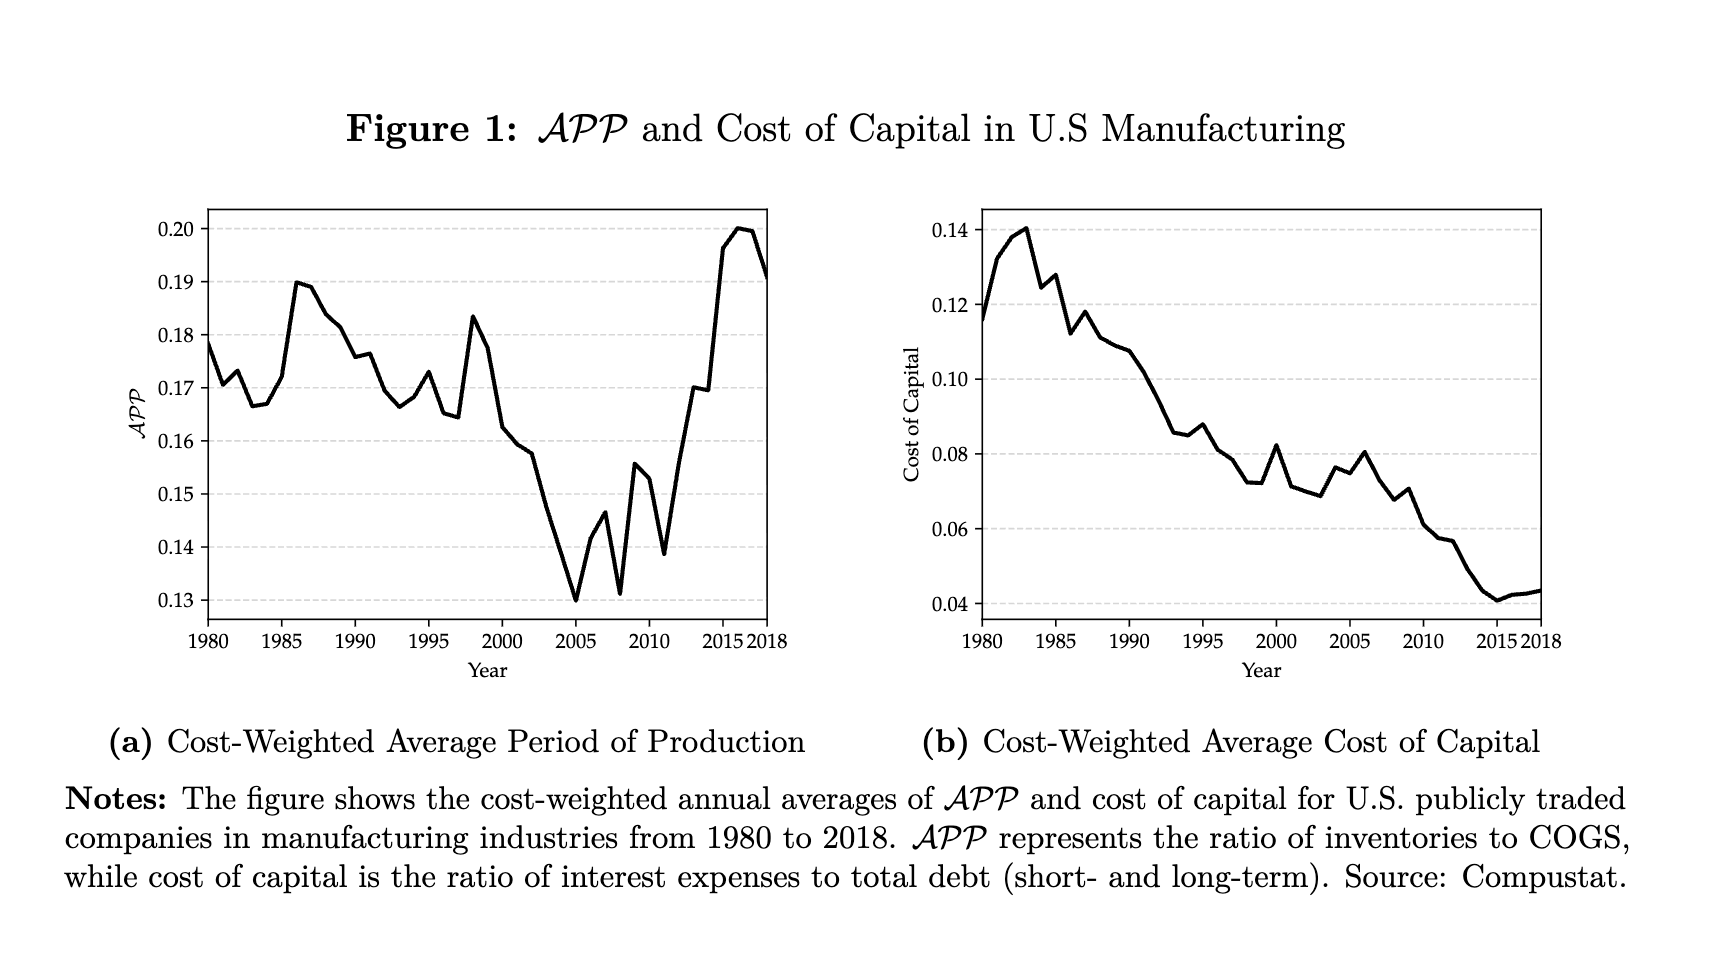
\includegraphics[width=1\linewidth]{Figure7.png}
\end{figure}
    
\end{frame}

\begin{frame}{Variation in the Average Period of Production Across Industries}
\begin{figure}
    \centering
    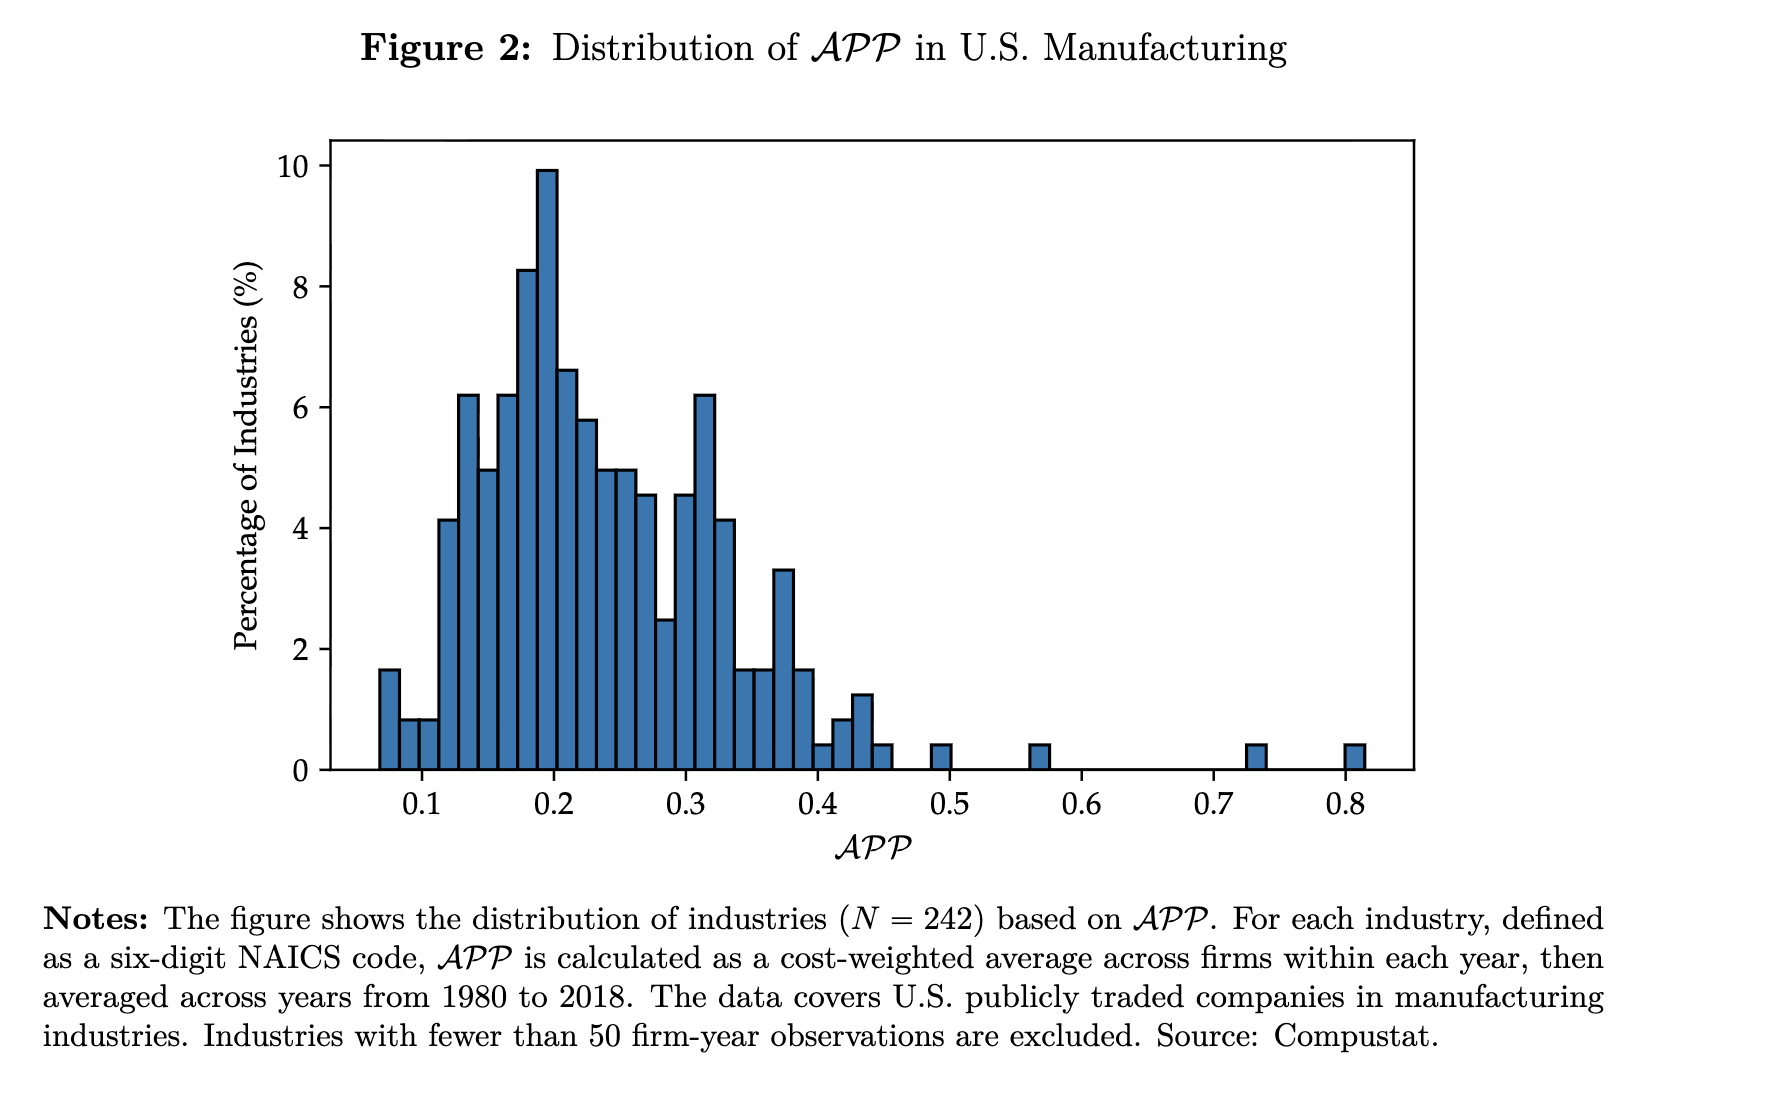
\includegraphics[width=1\linewidth]{Figure8.png}
\end{figure}

\end{frame}


\begin{frame}{Variation in the Average Period of Production Across Industries}
    \begin{figure}
        \centering
        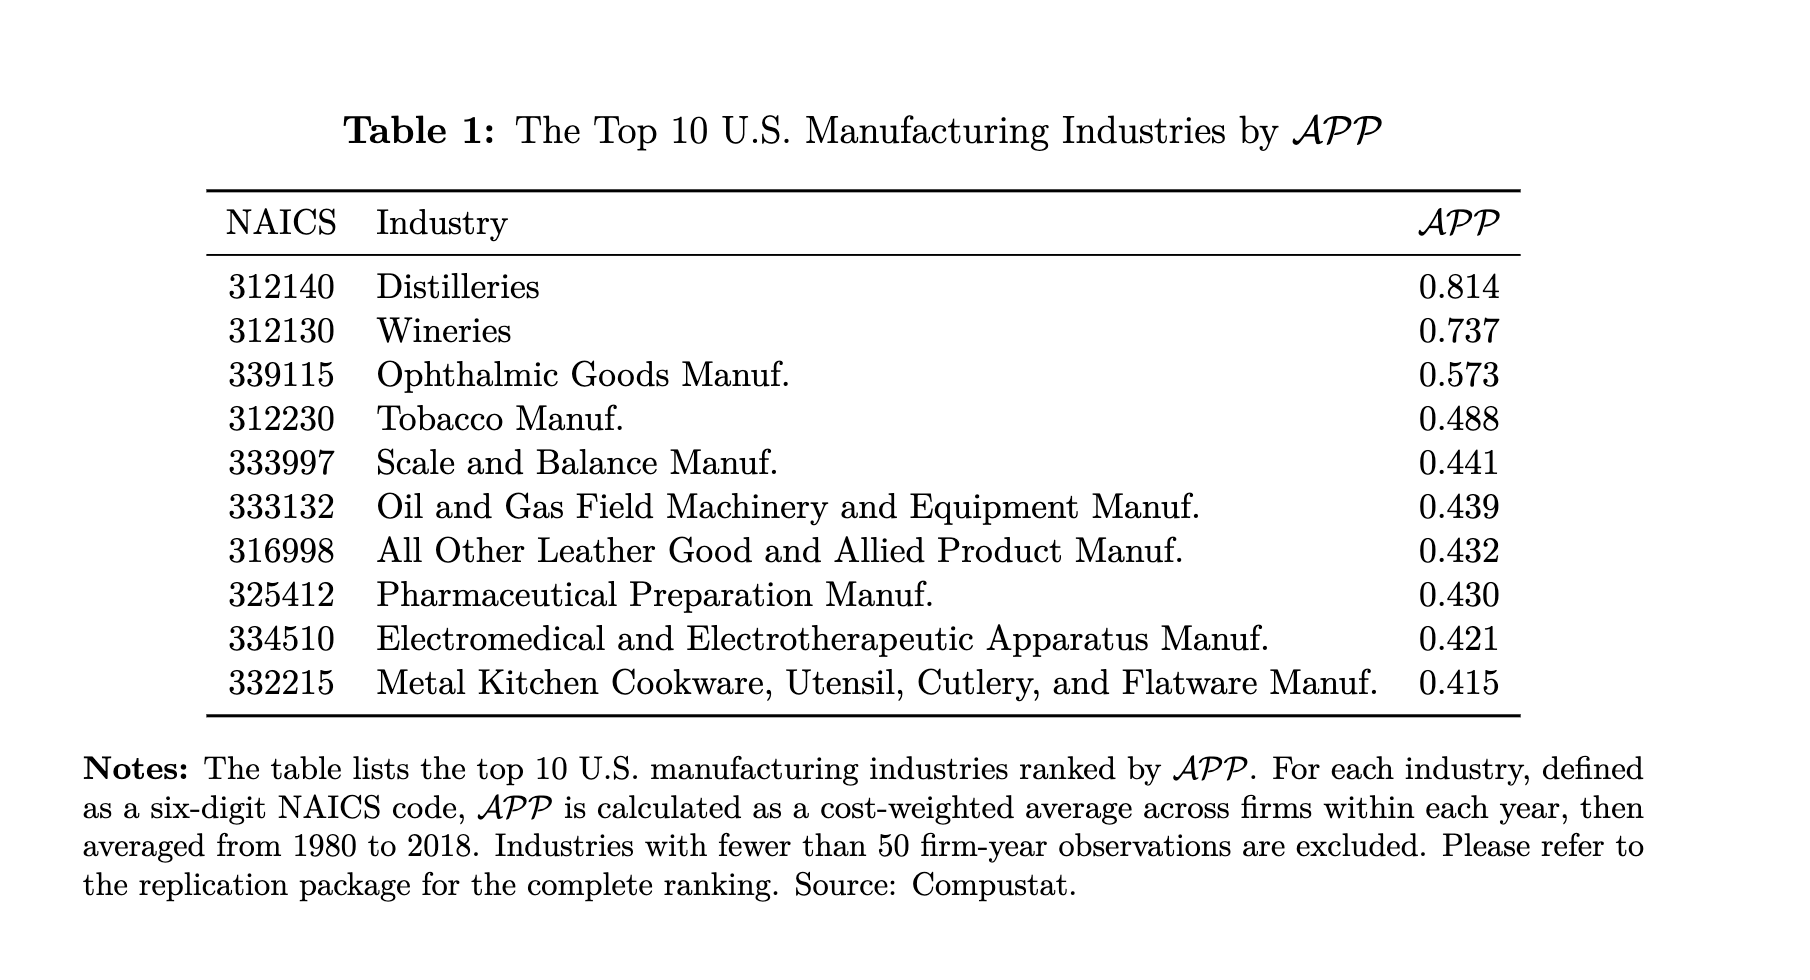
\includegraphics[width=1\linewidth]{Figure9.png}
    \end{figure}
\end{frame}

\begin{frame}{Variation in the Average Period of Production Across Industries}
\begin{figure}
    \centering
    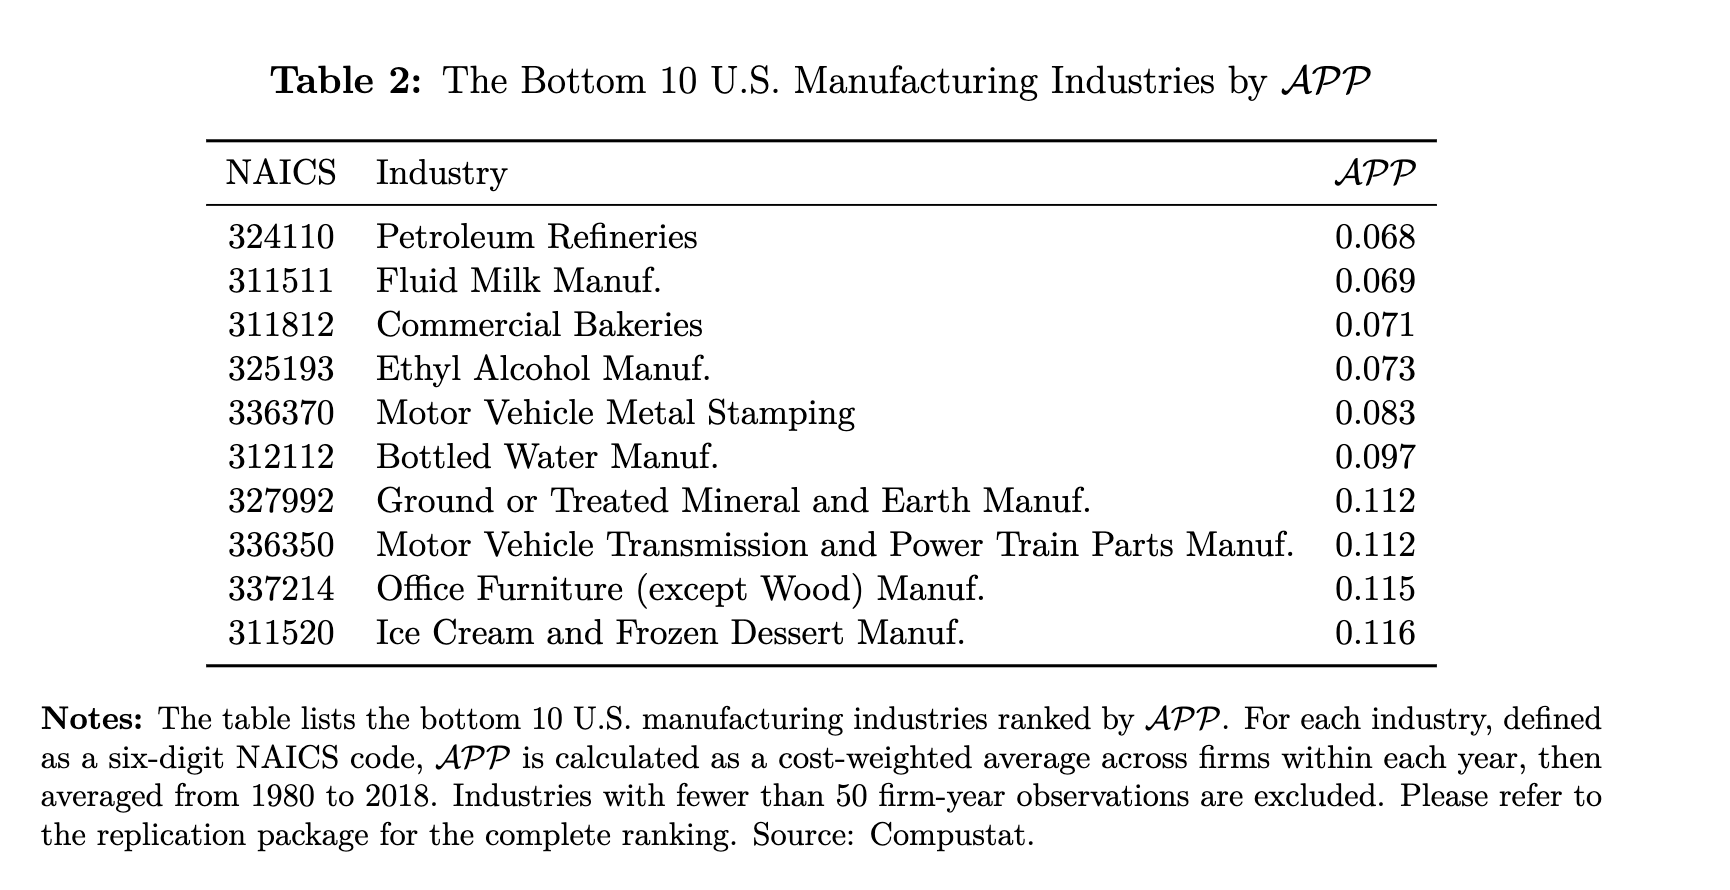
\includegraphics[width=1\linewidth]{Figure10.png}
\end{figure}
\end{frame}


\begin{frame}{The Average Period of Production and the Cost of Capital}
    $$\mathcal{APP}_{it} = \beta R_{it} + \gamma \mathbf{Z}_{it} + \mu_{i} + \lambda_{t} + \varepsilon_{it},$$
    \vspace{1cm}
    
    $R_{it}$ is the cost of capital faced by firm $i$ in year $t$
\end{frame}
\begin{frame}{The Average Period of Production and the Cost of Capital}
  \begin{figure}
      \centering
      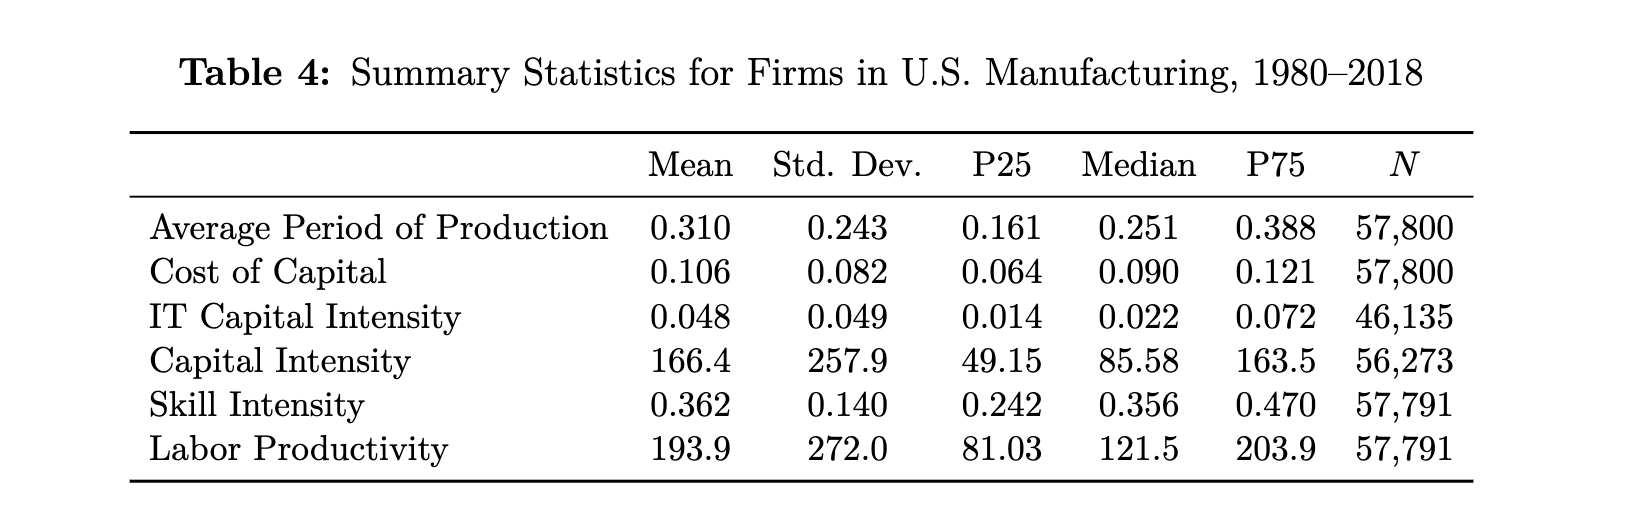
\includegraphics[width=1\linewidth]{Figure11.png}
  \end{figure}
\end{frame}


\begin{frame}{The Average Period of Production and the Cost of Capital}
    \begin{figure}
        \centering
        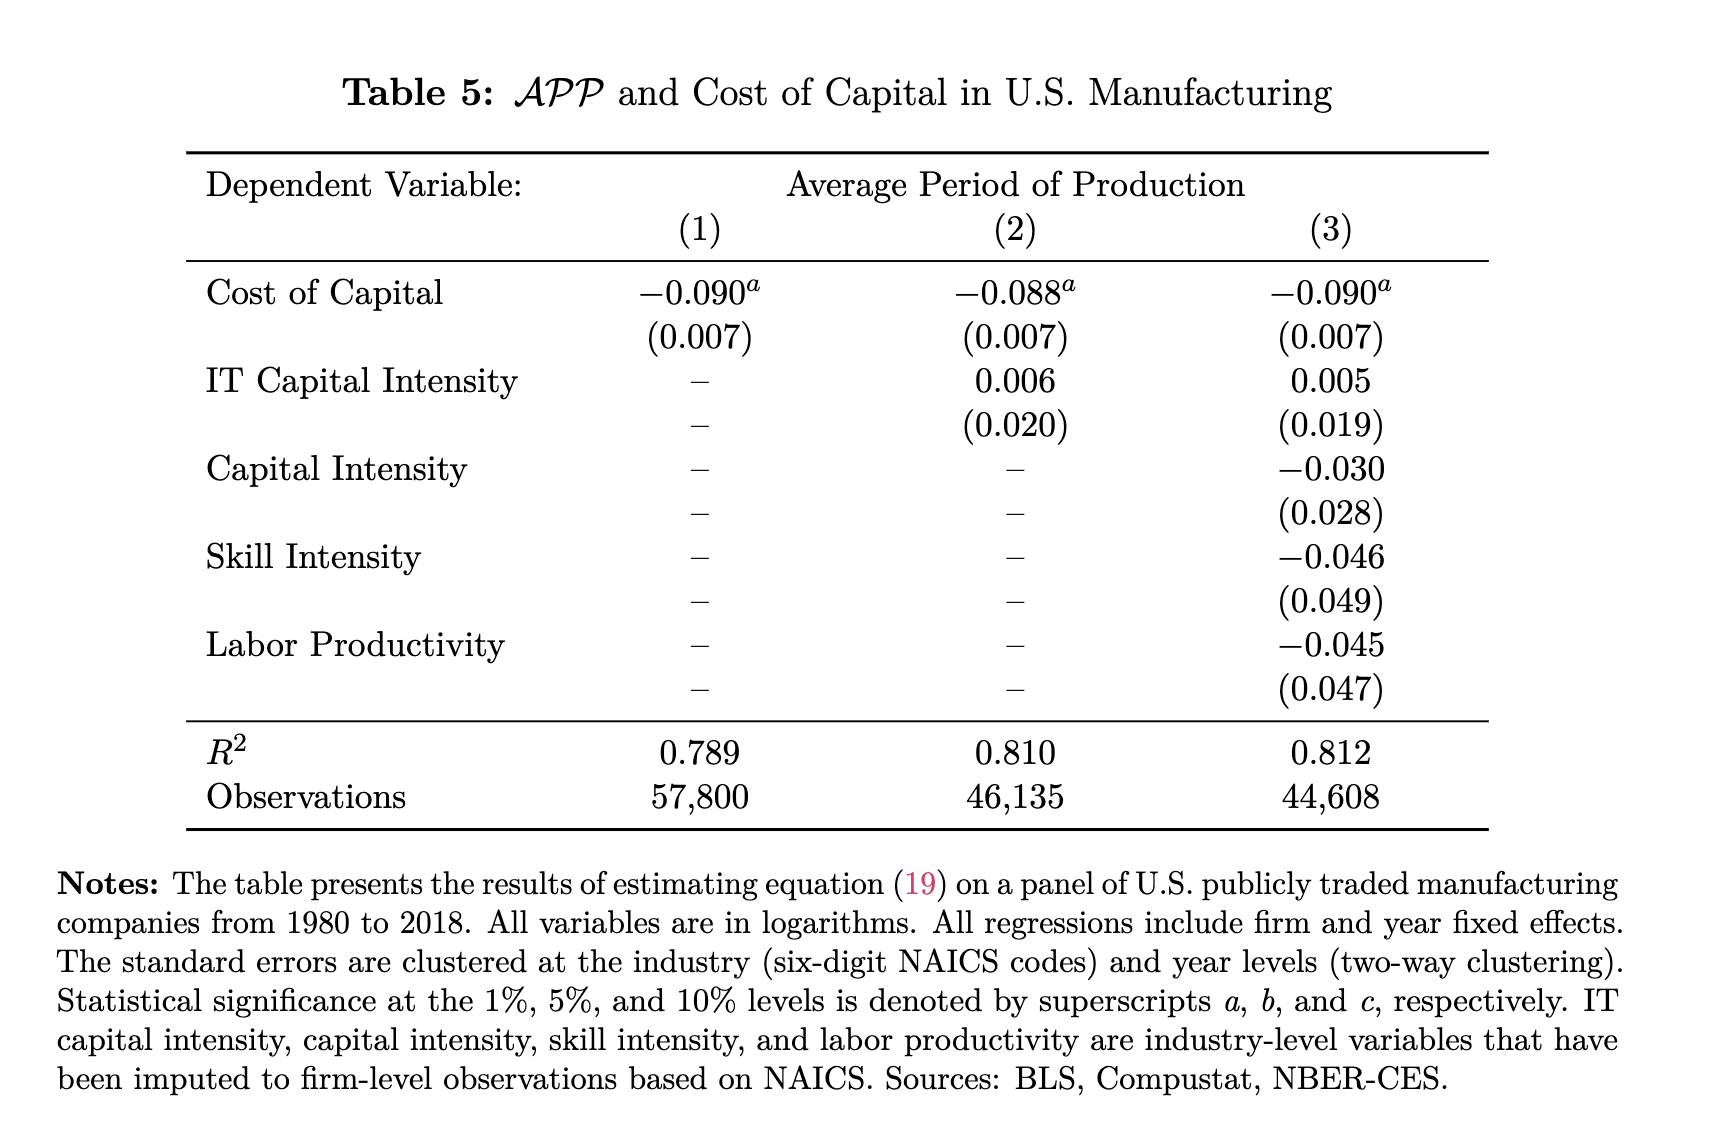
\includegraphics[width=1\linewidth]{Figure12.png}
    \end{figure}
\end{frame}

\begin{frame}{The Average Period of Production and the Cost of Capital}
    \begin{figure}
        \centering
        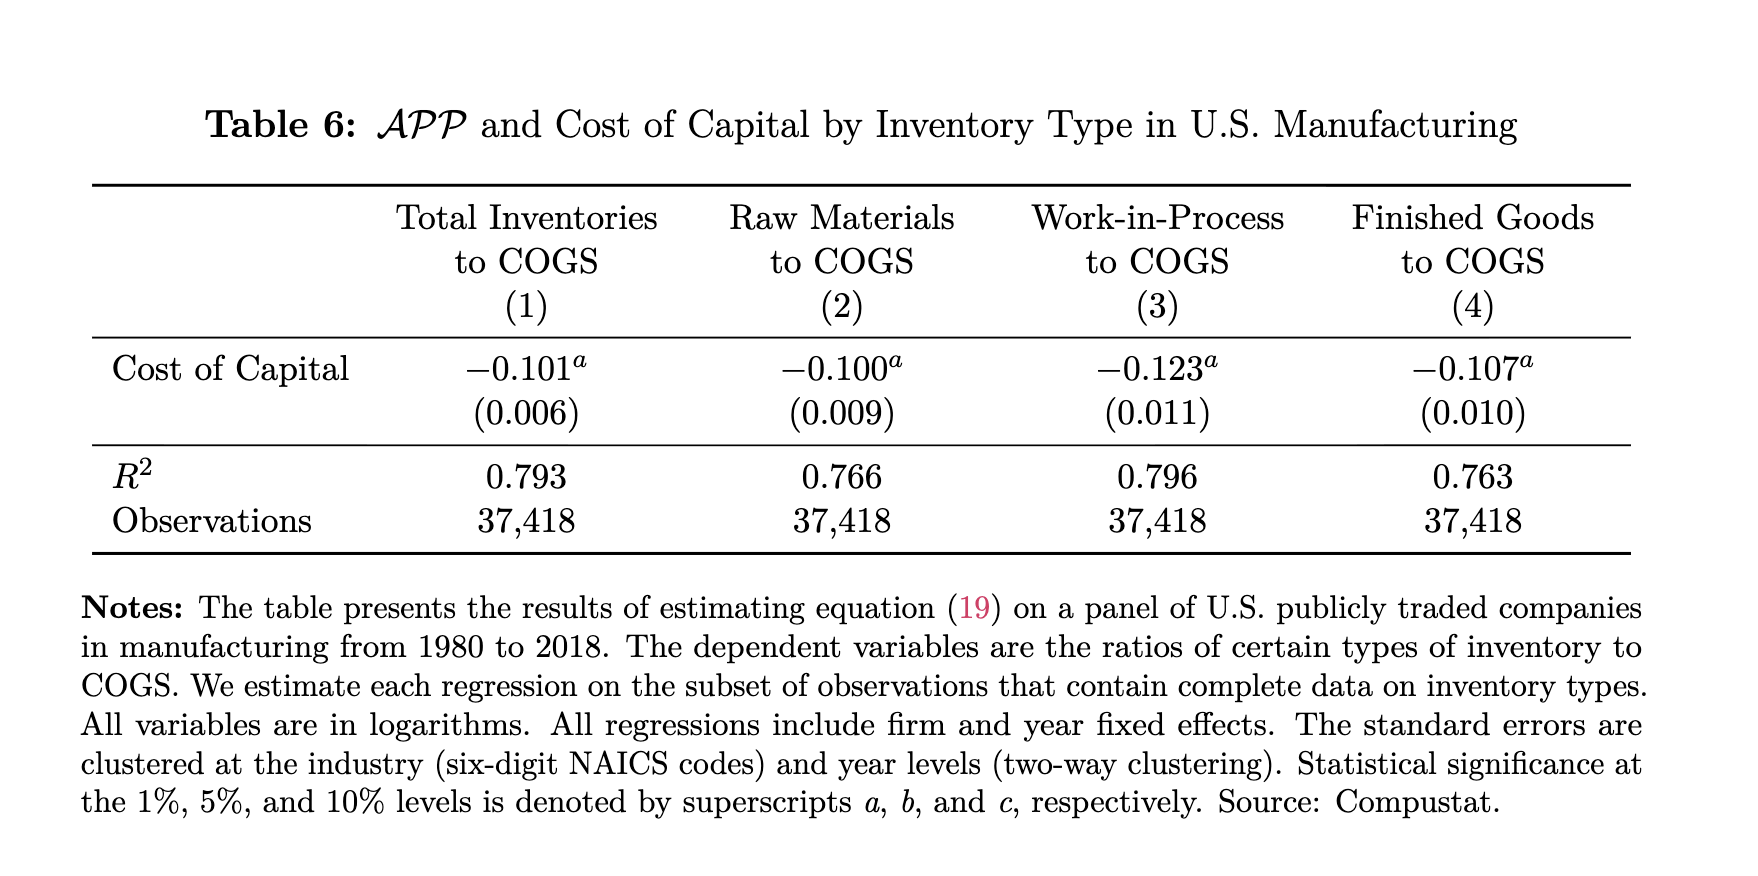
\includegraphics[width=1\linewidth]{Figure13.png}
    \end{figure}
\end{frame}

\begin{frame}
\centering
\Large The Average Period of Production Worldwide

    
\end{frame}

\begin{frame}{Rank Correlations of Industries}
  \begin{figure}
      \centering
      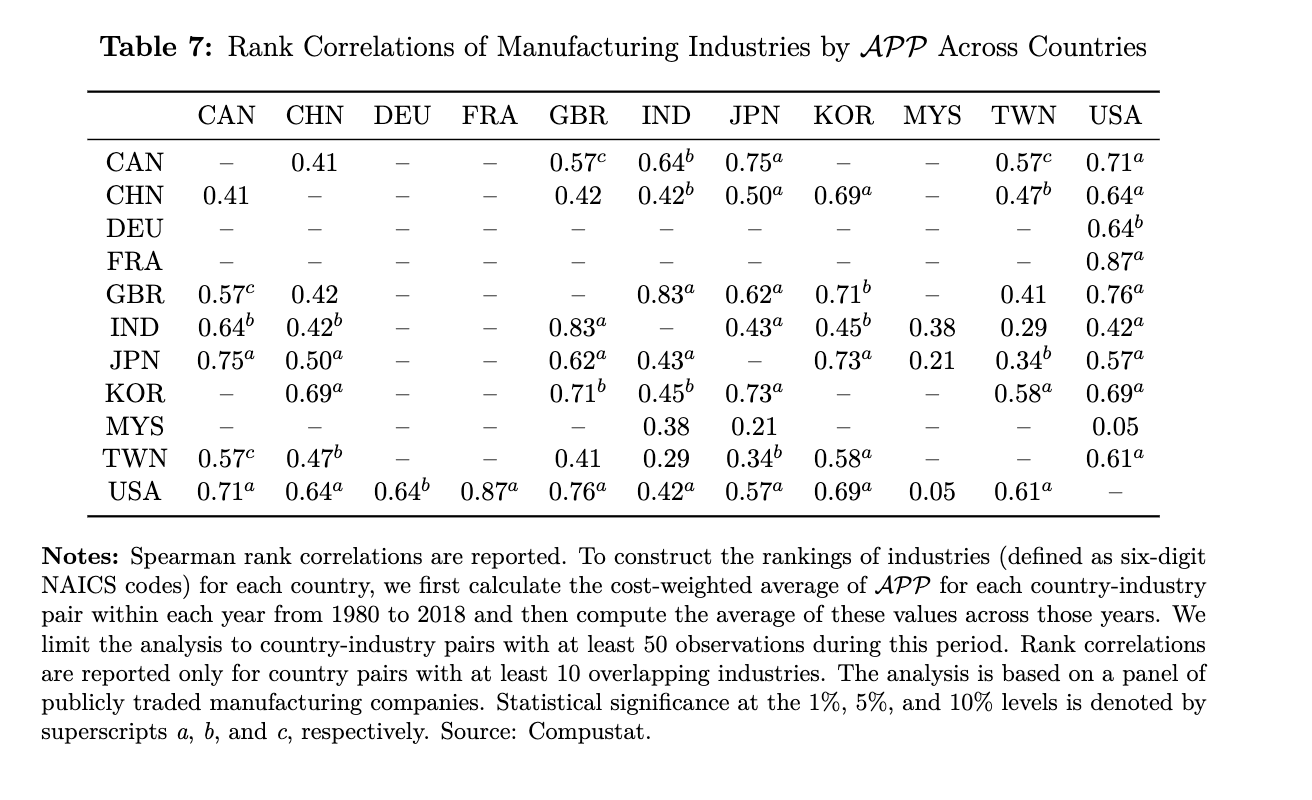
\includegraphics[width=1\linewidth]{image10.png}
  \end{figure}
\end{frame}

\begin{frame}{Pooled Regressions}
    \begin{figure}
        \centering
        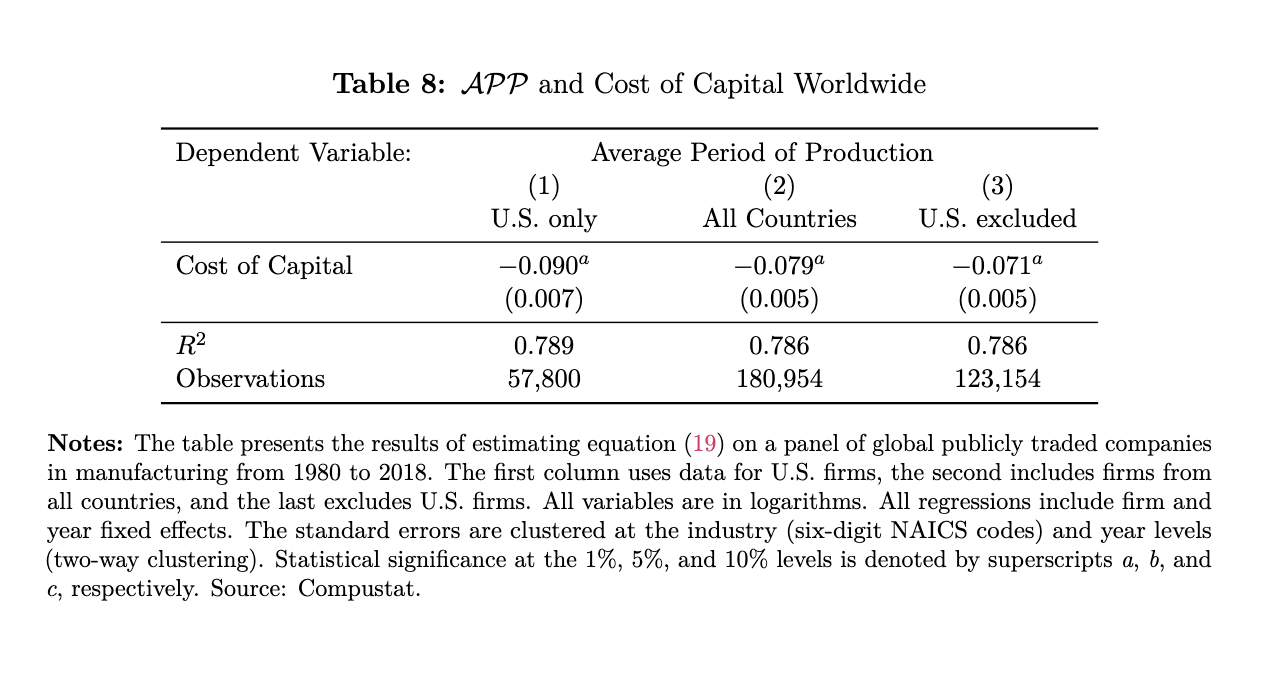
\includegraphics[width=1\linewidth]{image11.png}
    \end{figure}
\end{frame}



\begin{frame}{Heterogeneity at the Industry and Country Levels}
   \begin{figure}
       \centering
       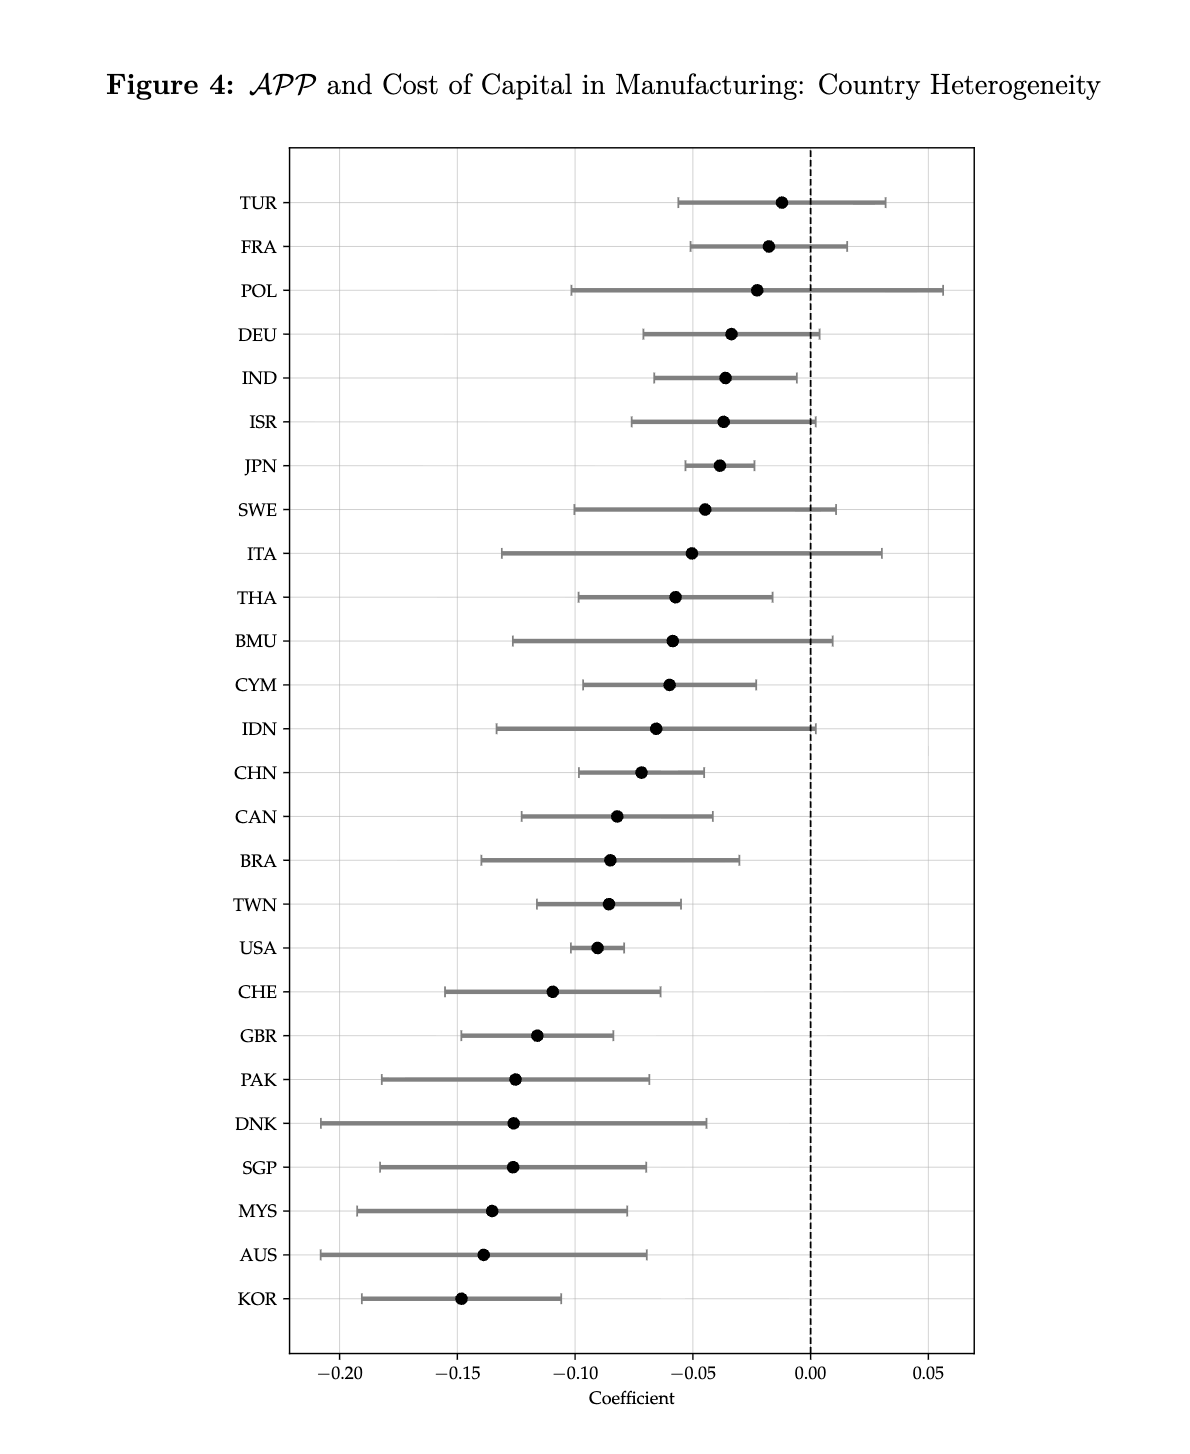
\includegraphics[width=.5\linewidth]{image12.png}
   \end{figure}
\end{frame}

\begin{frame}{Heterogeneity at the Industry and Country Levels}
    \begin{figure}
        \centering
        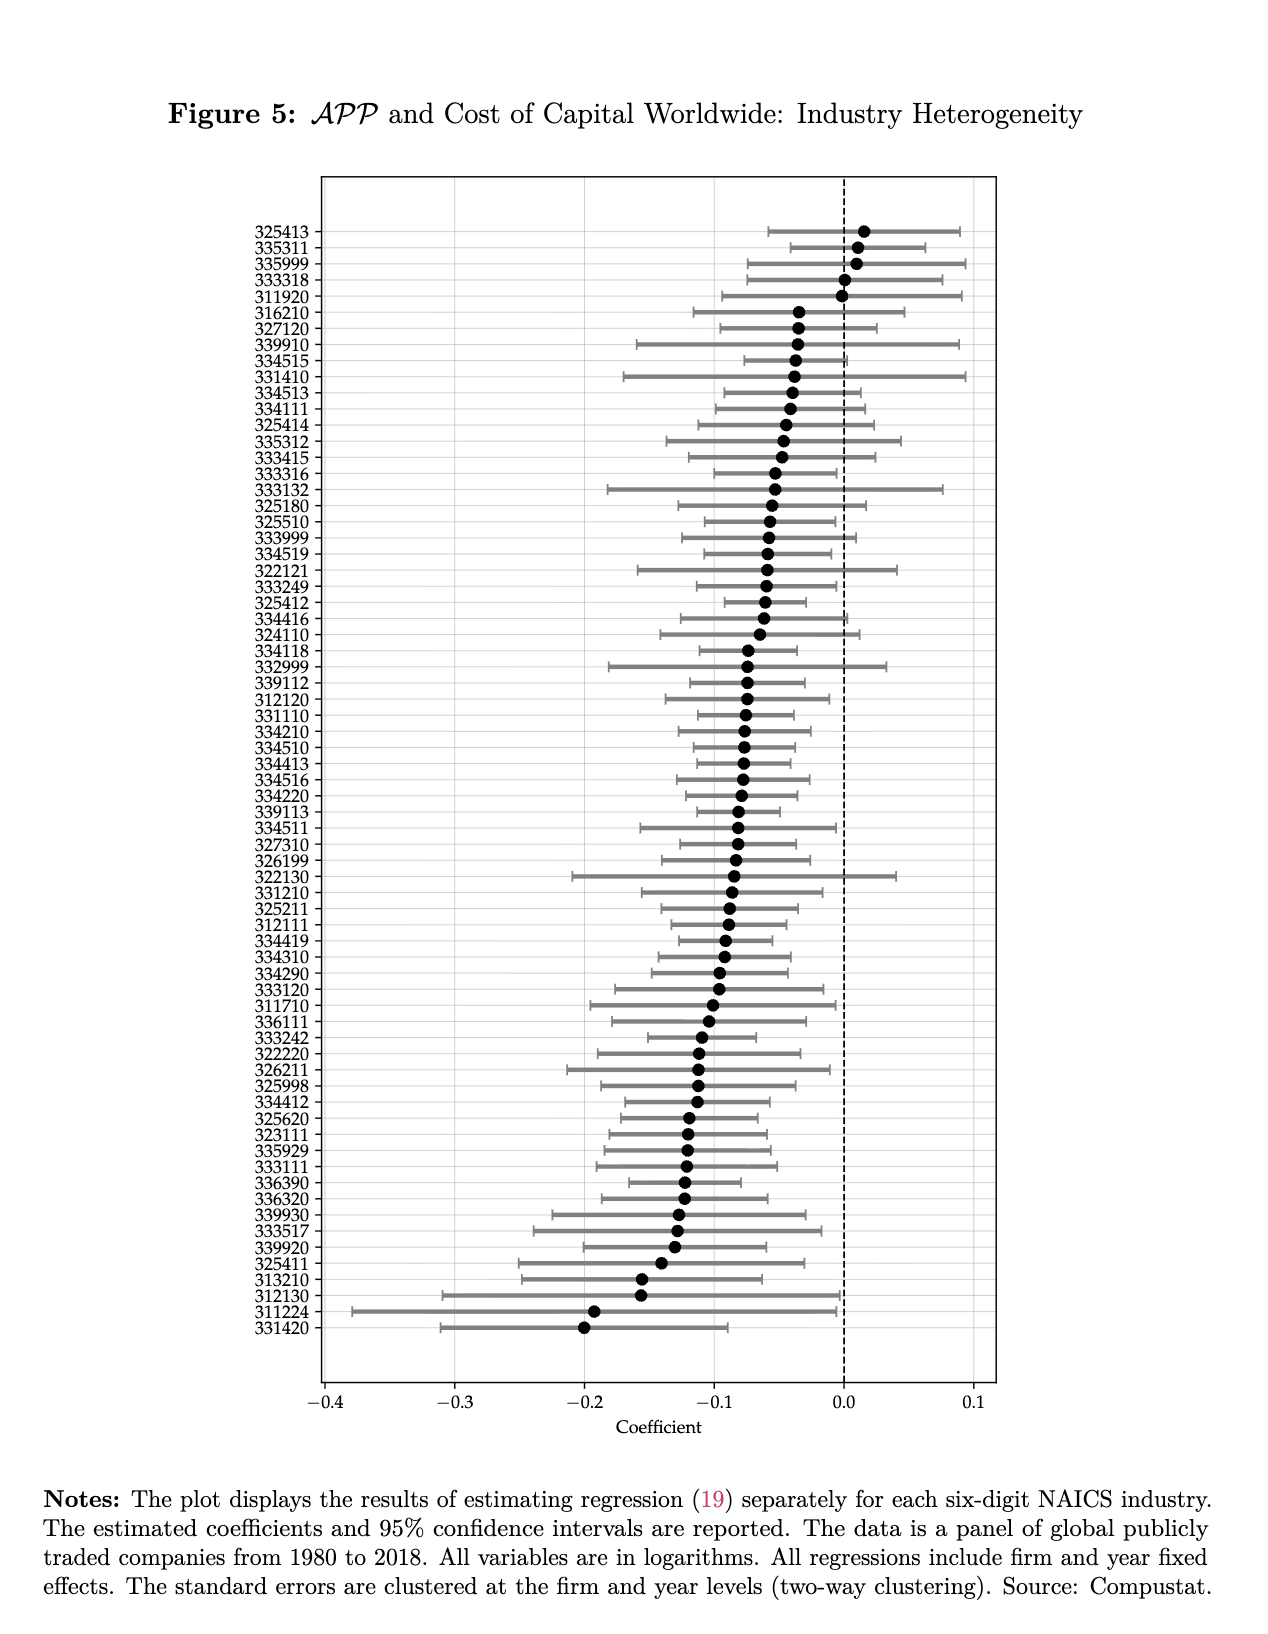
\includegraphics[width=.5\linewidth]{Figure14.png}
        \label{fig:placeholder}
    \end{figure}
\end{frame}
\begin{frame}{Conclusion}
\Large
Our ultimate aim is to foster further empirical research into how production length and
interest rates shape industrial structure.
    
\end{frame}


\begin{frame}
\centering
\huge (old Version) An ‘Austrian’ Model of Global Value Chains
    
\end{frame}

\begin{frame}{Baseline model}
\Large Building blocks
\begin{itemize}
    \item a sequential production process(Antràs and de Gortari (2020))
    \vspace{1cm}
    \item a temporal dimension to production (Findlay (1978))
    \vspace{1cm}
    \item to close the model, a supply side to the capital market(Antràs and Caballero (2009,2010))
\end{itemize}
    
\end{frame}

\begin{frame}{Environment}
\Large 
the population mass is constant and equal to $L$

\vspace{1cm}

All agents  are endowed with one unit of labor

\vspace{1cm}

Consumers value a single final good, which is taken to be the numéraire.

\end{frame}

\begin{frame}{Multi-stage production}
\Large
production of the single final good  needs to undergo N stages in a pre-determined, sequential order

\vspace{1cm}

At each stage $n>1$, production  combines labor with the good finished up to the previous stage $n-1$.

\vspace{1cm}

production in the initial  stage n 1 only uses labor


\end{frame}

\begin{frame}{Multi-stage production}
\Large
$$y_{n} = \left(z_{n} L_{n}\right)^{\alpha_{n}} \left(y_{n-1}\right)^{1-\alpha_{n}},$$
\vspace{1cm}
where $y_n$ is output after stage $n$ is performed.

$z_n$ denotes labor productivity at stage $n$
\vspace{1cm}

    
\end{frame}

\begin{frame}{Production takes time}
\Large
The main innovationis in acknowledging that production takes time.

\vspace{1cm}

the more time is devoted  to production, the more output will be obtained 

\vspace{1cm}
following the approach in Findlay (1978).
\end{frame}

\begin{frame}{Optimal production length}
\Large 
in stage 1

$$\pi_{1} = p_{1} z_{1}(t_{1}) L_{1} e^{-rt_{1}} - wL_{1}.$$

Firms treat good and factor prices as given, so $t_1$ will be set to maximize  profit

$$\frac{z_{1}^{\prime}(t_{1}^{*})}{z_{1}(t_{1}^{*})} = r.$$
\end{frame}

\begin{frame}{condition on $z_n(t)$}
\Large
How does productivity change over time.
    $$z_{n}^{\prime}(t) > 0$$
    $$\frac{z_{n}^{\prime\prime}(t)}{z_{n}^{\prime}(t)} < 0 < \frac{z_{n}^{\prime}(t)}{z_{n}(t)},$$
    \vspace{1cm}

to ensure the existence of a unique optimal.
$\frac{z_{n}^{\prime}(t_{1})}{z_{n}(t_{n})} \rightarrow \infty$ when $t_n \rightarrow 0$
$\frac{z_{n}^{\prime}(t_{1})}{z_{n}(t_{n})} \rightarrow 0$ when $t_n \rightarrow \infty$
\end{frame}

\begin{frame}{Optimal production length}
\Large
in stage $n$, producers pay wages and purchase the good finished up to the prior stage $n-1$

\vspace{1cm}

$$\pi_{n} = p_{n}\left(z_{n}(t_{n})L_{n}\right)^{\alpha_{n}}\left(y_{n-1}\right)^{1-\alpha_{n}}e^{-rt_{n}} - wL_{n} - p_{n-1}y_{n-1}.$$

\vspace{1cm}
then, the optimal stopping time $t^\ast_n$ will satisfy
$$\alpha_{n}\frac{z_{n}^{\prime}(t_{n}^{*})}{z_{n}(t_{n}^{*})} = r.$$
    
\end{frame}

\begin{frame}{Equilibrium Allocation of Labor Across Stages}
\Large 
Having solved all optimal production  lengths.

\vspace{1cm}

next solve for the allocation of labor across stages

    $$wL_{n}e^{rt_{n}} = \alpha_{n}p_{n}y_{n}$$
    $$p_{n-1}y_{n-1}e^{rt_{n}} = (1-\alpha_{n})p_{n}y_{n}.$$
\end{frame}


\begin{frame}{Equilibrium Allocation of Labor Across Stages}
\Large 
Iterating the second equation forward and plugging the result into the first one, delivers

$$wL_{n}e^{r\sum\limits_{m=n}^{N}t_{m}} = \alpha_{n}\beta_{n}y_{N},$$
where $\beta_{n} \equiv \prod_{m=n+1}^{N}\left(1-\alpha_{m}\right),$, $y_N$ is final output and final good revenue($p_N=1$)
\end{frame}

\begin{frame}{Equilibrium Allocation of Labor Across Stages}
according to production function:

$$y_{N} = \prod_{n=1}^{N}\left(z_{n}(t_{n})L_{n}\right)^{\alpha_{n}\beta_{n}}.$$

\vspace{1cm}
So, for any two stage $n^\prime>n $:
$$\frac{L_{n'}}{L_{n}} = \frac{\alpha_{n'}\beta_{n'}}{\alpha_{n}\beta_{n}}e^{r\sum\limits_{m=n}^{n'-1}t_{m}}.$$

\vspace{1cm}
SO GET!  Equilibrium allocation of labor across stages
\end{frame}

\begin{frame}{then}
\Large
\begin{enumerate}
    \item finish the closed economy version
    \item from close to open
    \item trade cost
    \item trade credit 
\end{enumerate}
    
\end{frame}

\begin{frame}
\centering

\huge 物流服务标准化与企业供应链地理布局

    
\end{frame}

\begin{frame}
\begin{itemize}
    \item 不同地区物流标准的混乱，带来高昂的物流成本,也制约了远距离企业之间的合作
    \vspace{1cm}
    \item 2014年逐步试点的物流标准化政策，以推进以托盘共用体系和建设物流综合信息服务平台为切入点，推进物流标准化工作（商务部和国家标准管理委员会，2014）。

\end{itemize}    
\end{frame}


\begin{frame}
    \begin{itemize}
    \item 借助中国2014年逐步试点的物流标准化政策，研究物流体系标准化对企业供应链地理布局的影响。
    \vspace{1cm}
    \item 机制：内，企业自身的经营成本，信息获取能力；外，优化地区的市场环境，市场一体化程度。
    \vspace{1cm}
    \item 进一步，企业的供应链风险，效率等；是否有供应链溢出。
    \end{itemize}
    
\end{frame}
\begin{frame}
\begin{figure}
    \centering
    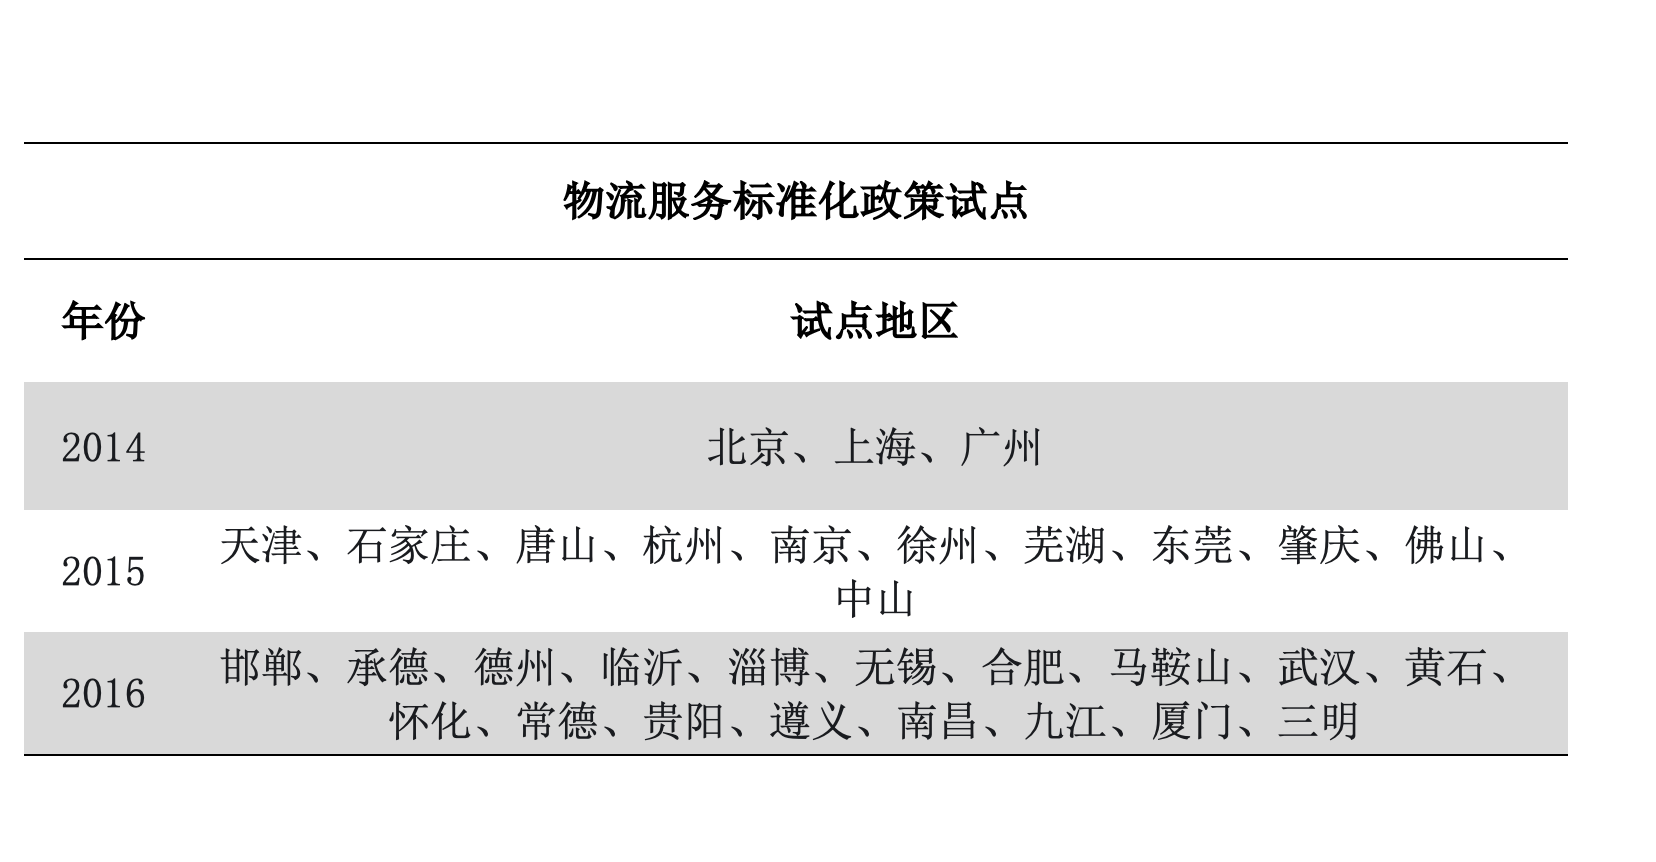
\includegraphics[width=1\linewidth]{image13.png}
\end{figure}
    
\end{frame}

\begin{frame}
为检验物流标准化政策对企业供应链地理地理分布的影响，设定如下交错型双重差分模型进行识别：
$$Disw\_S_{i,j,c,t} = \alpha + \beta Standard_{c,t} + \Gamma X_{i,t} + \delta_{i} + \lambda_{t} + \omega_{j,t} + \varepsilon_{i,j,c,t}$$
    $$Disw\_C_{i,j,c,t} = \alpha + \beta Standard_{c,t} + \Gamma X_{i,t} + \delta_{i} + \lambda_{t} + \omega_{j,t} + \varepsilon_{i,j,c,t}$$

\vspace{1cm}
    核心解释变量：物流标准化，以 2014年在城市层面分批实施的物流标准化试点政策作为准实验,构建核心解释变量：。当城市$c$在年份$t$被纳入物流标准化试点时, $Standard_{c,t}$在$t$及$t$年之后都赋值为1,否则为0。
    
    被解释变量：企业的供应链地理距离，以企业与前五大供应商和前五大客户的加权距离作为企业供应链地理距离的测度指标。
    $$Disw\_S_{it} = \ln\left(1 + \sum_{p} Dis\_S_{ipt} \times Ratio\_S_{ipt}\right)$$
       $$Disw\_C_{it} = \ln\left(1 + \sum_{p} Dis\_S_{ipt} \times Ratio\_S_{ipt}\right)$$
\end{frame}

\begin{frame}
    来源国泰安CSMAR数据库收集整理的2010-2024年A股上市公司数据作为研究样本。
    \begin{figure}
        \centering
        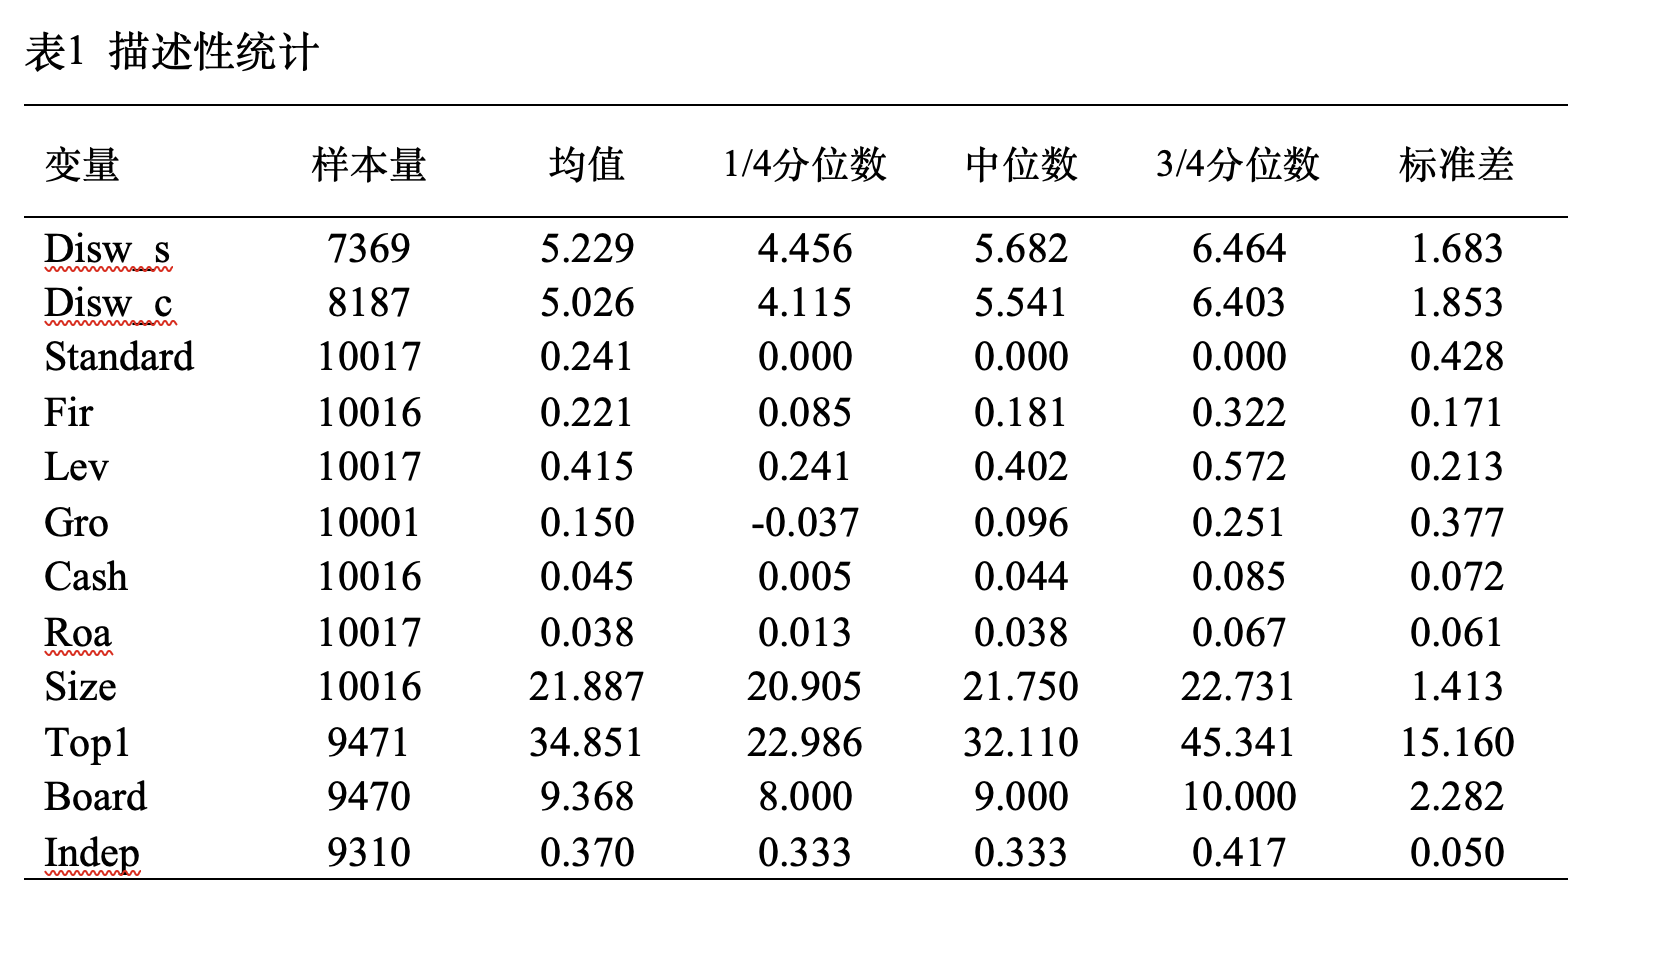
\includegraphics[width=1\linewidth]{image14.png}
    \end{figure}
\end{frame}

\begin{frame}
\begin{figure}
    \centering
    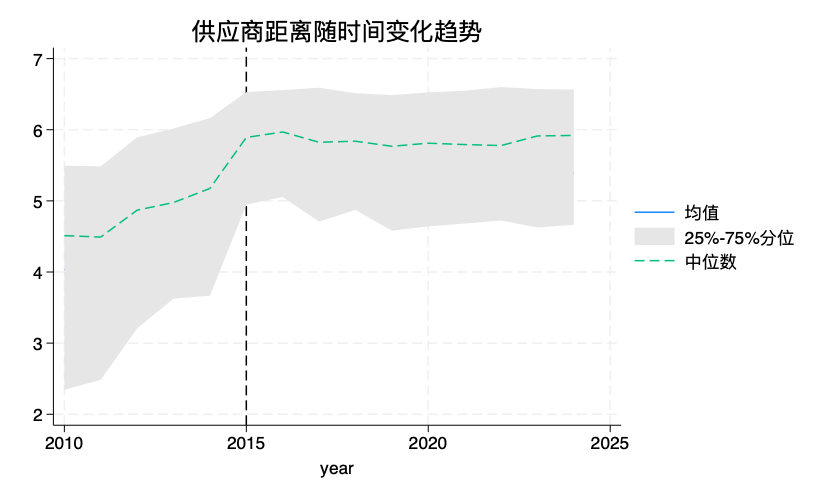
\includegraphics[width=1\linewidth]{image15.png}
\end{figure}
    
\end{frame}

\begin{frame}
\begin{figure}
    \centering
    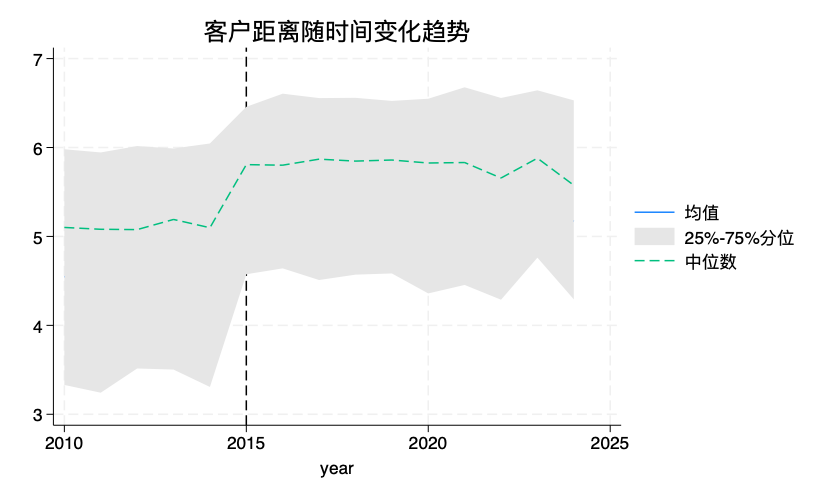
\includegraphics[width=1\linewidth]{image16.png}
\end{figure}
    
\end{frame}

\begin{frame}
\begin{figure}
    \centering
    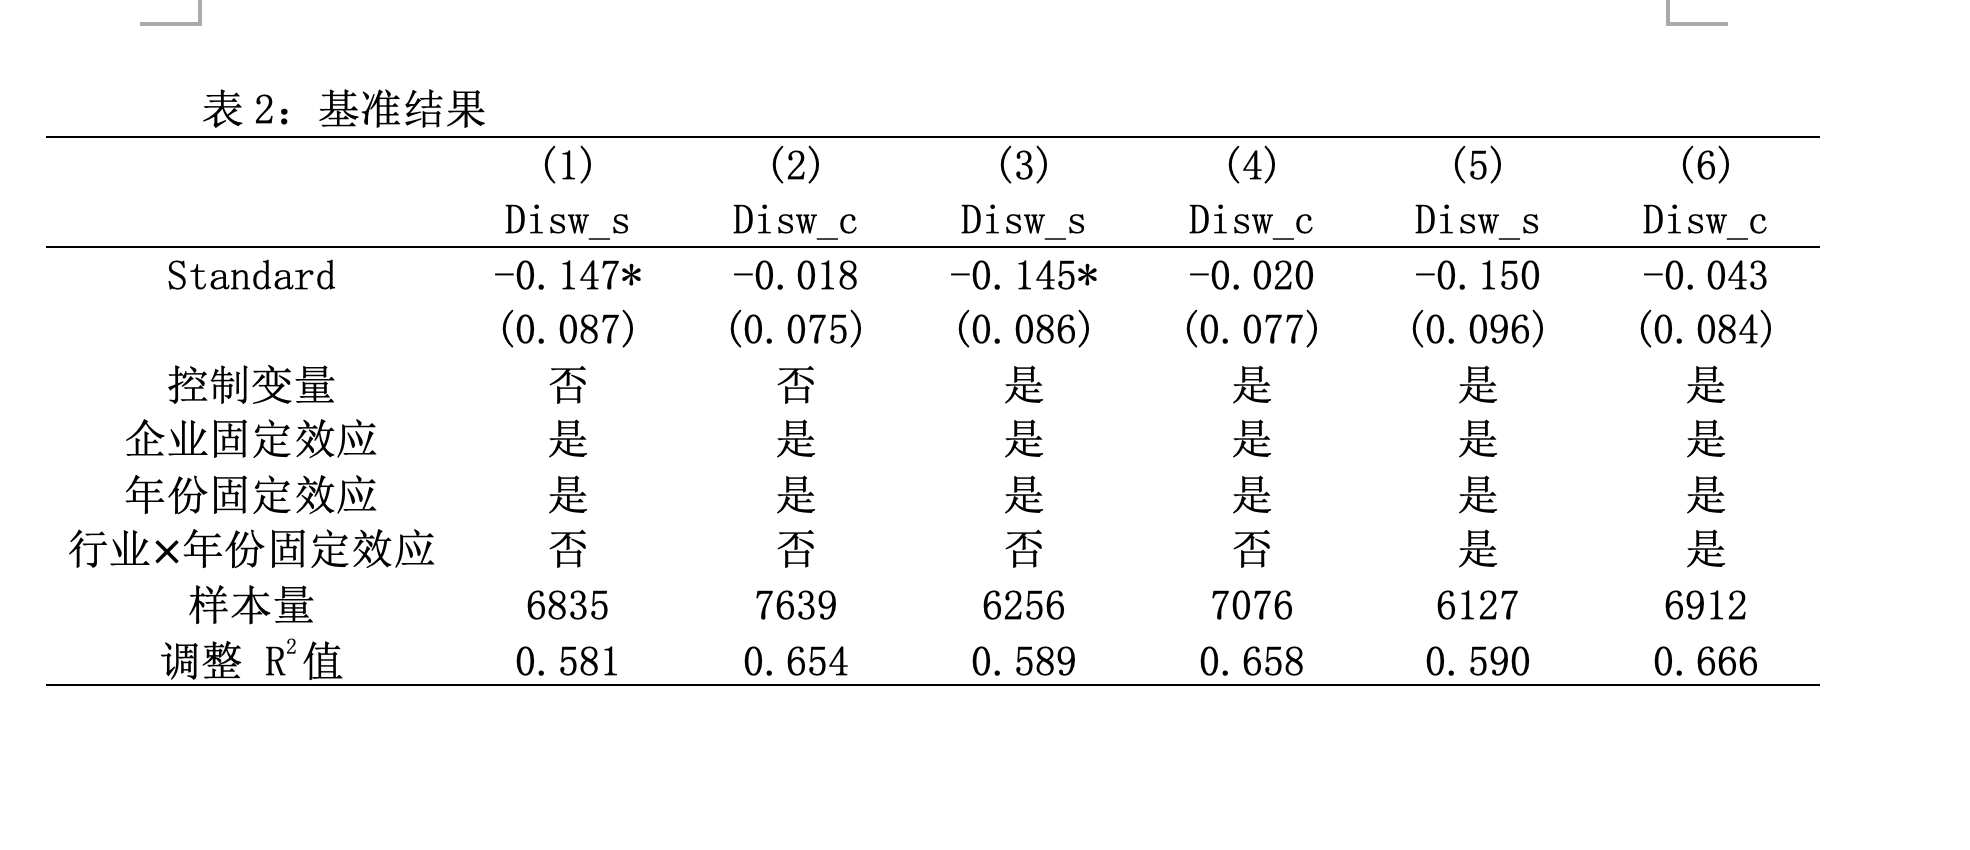
\includegraphics[width=1\linewidth]{1.png}
\end{figure}
    
\end{frame}

\begin{frame}
\begin{itemize}
    \item 数据缺失问题
    \vspace{1cm}
    \item 一种替代效应
    \vspace{1cm}
    \item 地方标准的市场分割
\end{itemize}
    
\end{frame}


\end{document}